% Created by tikzDevice version 0.11 on 2018-05-23 08:48:12
% !TEX encoding = UTF-8 Unicode
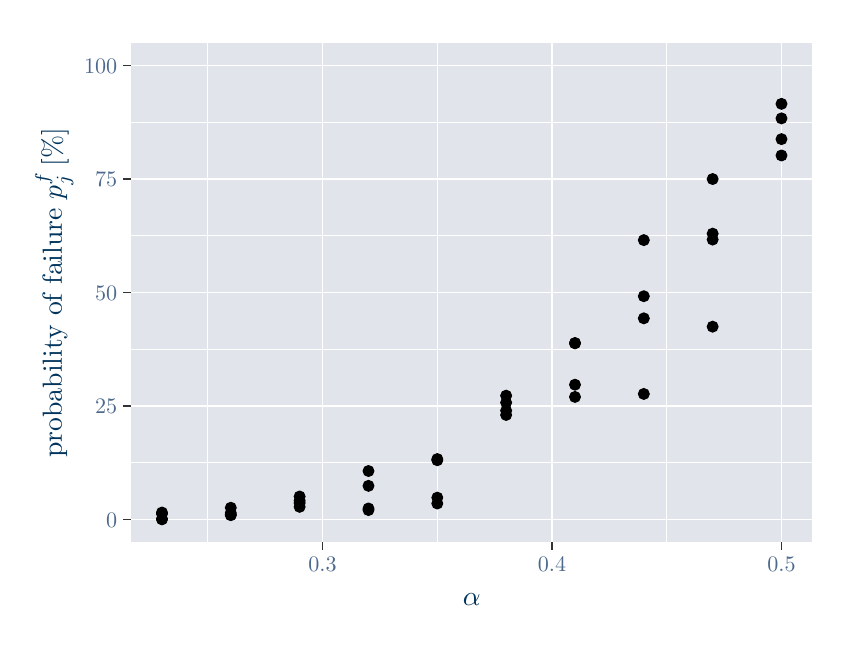
\begin{tikzpicture}[x=1pt,y=1pt]
\definecolor{fillColor}{RGB}{255,255,255}
\path[use as bounding box,fill=fillColor,fill opacity=0.00] (0,0) rectangle (289.08,216.81);
\begin{scope}
\path[clip] (  0.00,  0.00) rectangle (289.08,216.81);
\definecolor{drawColor}{RGB}{255,255,255}
\definecolor{fillColor}{RGB}{255,255,255}

\path[draw=drawColor,line width= 0.6pt,line join=round,line cap=round,fill=fillColor] (  0.00,  0.00) rectangle (289.08,216.81);
\end{scope}
\begin{scope}
\path[clip] ( 37.33, 30.85) rectangle (283.58,211.31);
\definecolor{fillColor}{RGB}{225,229,235}

\path[fill=fillColor] ( 37.33, 30.85) rectangle (283.58,211.31);
\definecolor{drawColor}{RGB}{255,255,255}

\path[draw=drawColor,line width= 0.3pt,line join=round] ( 37.33, 59.56) --
	(283.58, 59.56);

\path[draw=drawColor,line width= 0.3pt,line join=round] ( 37.33,100.57) --
	(283.58,100.57);

\path[draw=drawColor,line width= 0.3pt,line join=round] ( 37.33,141.59) --
	(283.58,141.59);

\path[draw=drawColor,line width= 0.3pt,line join=round] ( 37.33,182.60) --
	(283.58,182.60);

\path[draw=drawColor,line width= 0.3pt,line join=round] ( 65.11, 30.85) --
	( 65.11,211.31);

\path[draw=drawColor,line width= 0.3pt,line join=round] (148.02, 30.85) --
	(148.02,211.31);

\path[draw=drawColor,line width= 0.3pt,line join=round] (230.93, 30.85) --
	(230.93,211.31);

\path[draw=drawColor,line width= 0.6pt,line join=round] ( 37.33, 39.05) --
	(283.58, 39.05);

\path[draw=drawColor,line width= 0.6pt,line join=round] ( 37.33, 80.06) --
	(283.58, 80.06);

\path[draw=drawColor,line width= 0.6pt,line join=round] ( 37.33,121.08) --
	(283.58,121.08);

\path[draw=drawColor,line width= 0.6pt,line join=round] ( 37.33,162.09) --
	(283.58,162.09);

\path[draw=drawColor,line width= 0.6pt,line join=round] ( 37.33,203.11) --
	(283.58,203.11);

\path[draw=drawColor,line width= 0.6pt,line join=round] (106.56, 30.85) --
	(106.56,211.31);

\path[draw=drawColor,line width= 0.6pt,line join=round] (189.48, 30.85) --
	(189.48,211.31);

\path[draw=drawColor,line width= 0.6pt,line join=round] (272.39, 30.85) --
	(272.39,211.31);
\definecolor{drawColor}{RGB}{0,0,0}
\definecolor{fillColor}{RGB}{0,0,0}

\path[draw=drawColor,line width= 0.4pt,line join=round,line cap=round,fill=fillColor] ( 48.53, 41.61) circle (  1.96);

\path[draw=drawColor,line width= 0.4pt,line join=round,line cap=round,fill=fillColor] ( 73.40, 40.80) circle (  1.96);

\path[draw=drawColor,line width= 0.4pt,line join=round,line cap=round,fill=fillColor] ( 98.27, 45.90) circle (  1.96);

\path[draw=drawColor,line width= 0.4pt,line join=round,line cap=round,fill=fillColor] (123.15, 56.61) circle (  1.96);

\path[draw=drawColor,line width= 0.4pt,line join=round,line cap=round,fill=fillColor] (148.02, 46.99) circle (  1.96);

\path[draw=drawColor,line width= 0.4pt,line join=round,line cap=round,fill=fillColor] (172.89, 83.83) circle (  1.96);

\path[draw=drawColor,line width= 0.4pt,line join=round,line cap=round,fill=fillColor] (197.77, 87.80) circle (  1.96);

\path[draw=drawColor,line width= 0.4pt,line join=round,line cap=round,fill=fillColor] (222.64, 84.46) circle (  1.96);

\path[draw=drawColor,line width= 0.4pt,line join=round,line cap=round,fill=fillColor] (247.51,108.77) circle (  1.96);

\path[draw=drawColor,line width= 0.4pt,line join=round,line cap=round,fill=fillColor] (272.39,176.53) circle (  1.96);

\path[draw=drawColor,line width= 0.4pt,line join=round,line cap=round,fill=fillColor] ( 48.53, 39.15) circle (  1.96);

\path[draw=drawColor,line width= 0.4pt,line join=round,line cap=round,fill=fillColor] ( 73.40, 41.47) circle (  1.96);

\path[draw=drawColor,line width= 0.4pt,line join=round,line cap=round,fill=fillColor] ( 98.27, 43.66) circle (  1.96);

\path[draw=drawColor,line width= 0.4pt,line join=round,line cap=round,fill=fillColor] (123.15, 43.08) circle (  1.96);

\path[draw=drawColor,line width= 0.4pt,line join=round,line cap=round,fill=fillColor] (148.02, 60.50) circle (  1.96);

\path[draw=drawColor,line width= 0.4pt,line join=round,line cap=round,fill=fillColor] (172.89, 78.43) circle (  1.96);

\path[draw=drawColor,line width= 0.4pt,line join=round,line cap=round,fill=fillColor] (197.77,102.86) circle (  1.96);

\path[draw=drawColor,line width= 0.4pt,line join=round,line cap=round,fill=fillColor] (222.64,140.04) circle (  1.96);

\path[draw=drawColor,line width= 0.4pt,line join=round,line cap=round,fill=fillColor] (247.51,140.24) circle (  1.96);

\path[draw=drawColor,line width= 0.4pt,line join=round,line cap=round,fill=fillColor] (272.39,184.03) circle (  1.96);

\path[draw=drawColor,line width= 0.4pt,line join=round,line cap=round,fill=fillColor] ( 48.53, 41.15) circle (  1.96);

\path[draw=drawColor,line width= 0.4pt,line join=round,line cap=round,fill=fillColor] ( 73.40, 43.34) circle (  1.96);

\path[draw=drawColor,line width= 0.4pt,line join=round,line cap=round,fill=fillColor] ( 98.27, 45.03) circle (  1.96);

\path[draw=drawColor,line width= 0.4pt,line join=round,line cap=round,fill=fillColor] (123.15, 42.49) circle (  1.96);

\path[draw=drawColor,line width= 0.4pt,line join=round,line cap=round,fill=fillColor] (148.02, 44.87) circle (  1.96);

\path[draw=drawColor,line width= 0.4pt,line join=round,line cap=round,fill=fillColor] (172.89, 81.33) circle (  1.96);

\path[draw=drawColor,line width= 0.4pt,line join=round,line cap=round,fill=fillColor] (197.77, 83.38) circle (  1.96);

\path[draw=drawColor,line width= 0.4pt,line join=round,line cap=round,fill=fillColor] (222.64,119.77) circle (  1.96);

\path[draw=drawColor,line width= 0.4pt,line join=round,line cap=round,fill=fillColor] (247.51,142.38) circle (  1.96);

\path[draw=drawColor,line width= 0.4pt,line join=round,line cap=round,fill=fillColor] (272.39,170.63) circle (  1.96);

\path[draw=drawColor,line width= 0.4pt,line join=round,line cap=round,fill=fillColor] ( 48.53, 39.25) circle (  1.96);

\path[draw=drawColor,line width= 0.4pt,line join=round,line cap=round,fill=fillColor] ( 73.40, 40.64) circle (  1.96);

\path[draw=drawColor,line width= 0.4pt,line join=round,line cap=round,fill=fillColor] ( 98.27, 47.40) circle (  1.96);

\path[draw=drawColor,line width= 0.4pt,line join=round,line cap=round,fill=fillColor] (123.15, 51.25) circle (  1.96);

\path[draw=drawColor,line width= 0.4pt,line join=round,line cap=round,fill=fillColor] (148.02, 60.93) circle (  1.96);

\path[draw=drawColor,line width= 0.4pt,line join=round,line cap=round,fill=fillColor] (172.89, 76.86) circle (  1.96);

\path[draw=drawColor,line width= 0.4pt,line join=round,line cap=round,fill=fillColor] (197.77,102.75) circle (  1.96);

\path[draw=drawColor,line width= 0.4pt,line join=round,line cap=round,fill=fillColor] (222.64,111.78) circle (  1.96);

\path[draw=drawColor,line width= 0.4pt,line join=round,line cap=round,fill=fillColor] (247.51,162.11) circle (  1.96);

\path[draw=drawColor,line width= 0.4pt,line join=round,line cap=round,fill=fillColor] (272.39,189.28) circle (  1.96);
\end{scope}
\begin{scope}
\path[clip] (  0.00,  0.00) rectangle (289.08,216.81);
\definecolor{drawColor}{RGB}{77,106,141}

\node[text=drawColor,anchor=base east,inner sep=0pt, outer sep=0pt, scale=  0.80] at ( 32.38, 36.29) {0};

\node[text=drawColor,anchor=base east,inner sep=0pt, outer sep=0pt, scale=  0.80] at ( 32.38, 77.31) {25};

\node[text=drawColor,anchor=base east,inner sep=0pt, outer sep=0pt, scale=  0.80] at ( 32.38,118.32) {50};

\node[text=drawColor,anchor=base east,inner sep=0pt, outer sep=0pt, scale=  0.80] at ( 32.38,159.34) {75};

\node[text=drawColor,anchor=base east,inner sep=0pt, outer sep=0pt, scale=  0.80] at ( 32.38,200.35) {100};
\end{scope}
\begin{scope}
\path[clip] (  0.00,  0.00) rectangle (289.08,216.81);
\definecolor{drawColor}{gray}{0.20}

\path[draw=drawColor,line width= 0.6pt,line join=round] ( 34.58, 39.05) --
	( 37.33, 39.05);

\path[draw=drawColor,line width= 0.6pt,line join=round] ( 34.58, 80.06) --
	( 37.33, 80.06);

\path[draw=drawColor,line width= 0.6pt,line join=round] ( 34.58,121.08) --
	( 37.33,121.08);

\path[draw=drawColor,line width= 0.6pt,line join=round] ( 34.58,162.09) --
	( 37.33,162.09);

\path[draw=drawColor,line width= 0.6pt,line join=round] ( 34.58,203.11) --
	( 37.33,203.11);
\end{scope}
\begin{scope}
\path[clip] (  0.00,  0.00) rectangle (289.08,216.81);
\definecolor{drawColor}{gray}{0.20}

\path[draw=drawColor,line width= 0.6pt,line join=round] (106.56, 28.10) --
	(106.56, 30.85);

\path[draw=drawColor,line width= 0.6pt,line join=round] (189.48, 28.10) --
	(189.48, 30.85);

\path[draw=drawColor,line width= 0.6pt,line join=round] (272.39, 28.10) --
	(272.39, 30.85);
\end{scope}
\begin{scope}
\path[clip] (  0.00,  0.00) rectangle (289.08,216.81);
\definecolor{drawColor}{RGB}{77,106,141}

\node[text=drawColor,anchor=base,inner sep=0pt, outer sep=0pt, scale=  0.80] at (106.56, 20.39) {0.3};

\node[text=drawColor,anchor=base,inner sep=0pt, outer sep=0pt, scale=  0.80] at (189.48, 20.39) {0.4};

\node[text=drawColor,anchor=base,inner sep=0pt, outer sep=0pt, scale=  0.80] at (272.39, 20.39) {0.5};
\end{scope}
\begin{scope}
\path[clip] (  0.00,  0.00) rectangle (289.08,216.81);
\definecolor{drawColor}{RGB}{0,52,92}

\node[text=drawColor,anchor=base,inner sep=0pt, outer sep=0pt, scale=  1.00] at (160.46,  8.00) {$\alpha$};
\end{scope}
\begin{scope}
\path[clip] (  0.00,  0.00) rectangle (289.08,216.81);
\definecolor{drawColor}{RGB}{0,52,92}

\node[text=drawColor,rotate= 90.00,anchor=base,inner sep=0pt, outer sep=0pt, scale=  1.00] at ( 12.39,121.08) {probability of failure $p^f_j \left[\%\right]$};
\end{scope}
\end{tikzpicture}
